\documentclass[twoside]{book}

% Packages required by doxygen
\usepackage{fixltx2e}
\usepackage{calc}
\usepackage{doxygen}
\usepackage[export]{adjustbox} % also loads graphicx
\usepackage{graphicx}
\usepackage[utf8]{inputenc}
\usepackage{makeidx}
\usepackage{multicol}
\usepackage{multirow}
\PassOptionsToPackage{warn}{textcomp}
\usepackage{textcomp}
\usepackage[nointegrals]{wasysym}
\usepackage[table]{xcolor}

% Font selection
\usepackage[T1]{fontenc}
\usepackage[scaled=.90]{helvet}
\usepackage{courier}
\usepackage{amssymb}
\usepackage{sectsty}
\renewcommand{\familydefault}{\sfdefault}
\allsectionsfont{%
  \fontseries{bc}\selectfont%
  \color{darkgray}%
}
\renewcommand{\DoxyLabelFont}{%
  \fontseries{bc}\selectfont%
  \color{darkgray}%
}
\newcommand{\+}{\discretionary{\mbox{\scriptsize$\hookleftarrow$}}{}{}}

% Page & text layout
\usepackage{geometry}
\geometry{%
  a4paper,%
  top=2.5cm,%
  bottom=2.5cm,%
  left=2.5cm,%
  right=2.5cm%
}
\tolerance=750
\hfuzz=15pt
\hbadness=750
\setlength{\emergencystretch}{15pt}
\setlength{\parindent}{0cm}
\setlength{\parskip}{3ex plus 2ex minus 2ex}
\makeatletter
\renewcommand{\paragraph}{%
  \@startsection{paragraph}{4}{0ex}{-1.0ex}{1.0ex}{%
    \normalfont\normalsize\bfseries\SS@parafont%
  }%
}
\renewcommand{\subparagraph}{%
  \@startsection{subparagraph}{5}{0ex}{-1.0ex}{1.0ex}{%
    \normalfont\normalsize\bfseries\SS@subparafont%
  }%
}
\makeatother

% Headers & footers
\usepackage{fancyhdr}
\pagestyle{fancyplain}
\fancyhead[LE]{\fancyplain{}{\bfseries\thepage}}
\fancyhead[CE]{\fancyplain{}{}}
\fancyhead[RE]{\fancyplain{}{\bfseries\leftmark}}
\fancyhead[LO]{\fancyplain{}{\bfseries\rightmark}}
\fancyhead[CO]{\fancyplain{}{}}
\fancyhead[RO]{\fancyplain{}{\bfseries\thepage}}
\fancyfoot[LE]{\fancyplain{}{}}
\fancyfoot[CE]{\fancyplain{}{}}
\fancyfoot[RE]{\fancyplain{}{\bfseries\scriptsize Generated by Doxygen }}
\fancyfoot[LO]{\fancyplain{}{\bfseries\scriptsize Generated by Doxygen }}
\fancyfoot[CO]{\fancyplain{}{}}
\fancyfoot[RO]{\fancyplain{}{}}
\renewcommand{\footrulewidth}{0.4pt}
\renewcommand{\chaptermark}[1]{%
  \markboth{#1}{}%
}
\renewcommand{\sectionmark}[1]{%
  \markright{\thesection\ #1}%
}

% Indices & bibliography
\usepackage{natbib}
\usepackage[titles]{tocloft}
\setcounter{tocdepth}{3}
\setcounter{secnumdepth}{5}
\makeindex

% Hyperlinks (required, but should be loaded last)
\usepackage{ifpdf}
\ifpdf
  \usepackage[pdftex,pagebackref=true]{hyperref}
\else
  \usepackage[ps2pdf,pagebackref=true]{hyperref}
\fi
\hypersetup{%
  colorlinks=true,%
  linkcolor=blue,%
  citecolor=blue,%
  unicode%
}

% Custom commands
\newcommand{\clearemptydoublepage}{%
  \newpage{\pagestyle{empty}\cleardoublepage}%
}

\usepackage{caption}
\captionsetup{labelsep=space,justification=centering,font={bf},singlelinecheck=off,skip=4pt,position=top}

%===== C O N T E N T S =====

\begin{document}

% Titlepage & ToC
\hypersetup{pageanchor=false,
             bookmarksnumbered=true,
             pdfencoding=unicode
            }
\pagenumbering{alph}
\begin{titlepage}
\vspace*{7cm}
\begin{center}%
{\Large Queue\+A\+D\+T.\+h }\\
\vspace*{1cm}
{\large Generated by Doxygen 1.8.13}\\
\end{center}
\end{titlepage}
\clearemptydoublepage
\pagenumbering{roman}
\tableofcontents
\clearemptydoublepage
\pagenumbering{arabic}
\hypersetup{pageanchor=true}

%--- Begin generated contents ---
\chapter{Class Index}
\section{Class List}
Here are the classes, structs, unions and interfaces with brief descriptions\+:\begin{DoxyCompactList}
\item\contentsline{section}{\hyperlink{structHeap}{Heap} }{\pageref{structHeap}}{}
\item\contentsline{section}{\hyperlink{structNode}{Node} }{\pageref{structNode}}{}
\end{DoxyCompactList}

\chapter{File Index}
\section{File List}
Here is a list of all documented files with brief descriptions\+:\begin{DoxyCompactList}
\item\contentsline{section}{include/\hyperlink{car_8h}{car.\+h} \\*File containing the function definitions needed for car struct }{\pageref{car_8h}}{}
\end{DoxyCompactList}

\chapter{Class Documentation}
\hypertarget{structqueue}{}\section{queue Struct Reference}
\label{structqueue}\index{queue@{queue}}


{\ttfamily \#include $<$Queue\+A\+D\+T.\+h$>$}

\subsection*{Public Attributes}
\begin{DoxyCompactItemize}
\item 
\mbox{\Hypertarget{structqueue_adc9a0c20099370037a33607c9aa8d263}\label{structqueue_adc9a0c20099370037a33607c9aa8d263}} 
List $\ast$ {\bfseries list}
\item 
\mbox{\Hypertarget{structqueue_a1a583a22b96c1b91194cb1e02446d7ab}\label{structqueue_a1a583a22b96c1b91194cb1e02446d7ab}} 
Node $\ast$ {\bfseries front}
\item 
\mbox{\Hypertarget{structqueue_af2ce721719789280f495041c8151a445}\label{structqueue_af2ce721719789280f495041c8151a445}} 
int {\bfseries length}
\end{DoxyCompactItemize}


\subsection{Detailed Description}
Queue. It contains a list pointer, a node pointer that points to the front of the queue and length that determines number of elements. 

The documentation for this struct was generated from the following file\+:\begin{DoxyCompactItemize}
\item 
include/\hyperlink{QueueADT_8h}{Queue\+A\+D\+T.\+h}\end{DoxyCompactItemize}

\chapter{File Documentation}
\hypertarget{QueueADT_8h}{}\section{include/\+Queue\+A\+DT.h File Reference}
\label{QueueADT_8h}\index{include/\+Queue\+A\+D\+T.\+h@{include/\+Queue\+A\+D\+T.\+h}}


File containing the function definitions of a queue wrapping a doubly linked list.  


{\ttfamily \#include $<$stdio.\+h$>$}\newline
{\ttfamily \#include $<$stdlib.\+h$>$}\newline
{\ttfamily \#include \char`\"{}Linked\+List\+A\+P\+I.\+h\char`\"{}}\newline
Include dependency graph for Queue\+A\+D\+T.\+h\+:
\nopagebreak
\begin{figure}[H]
\begin{center}
\leavevmode
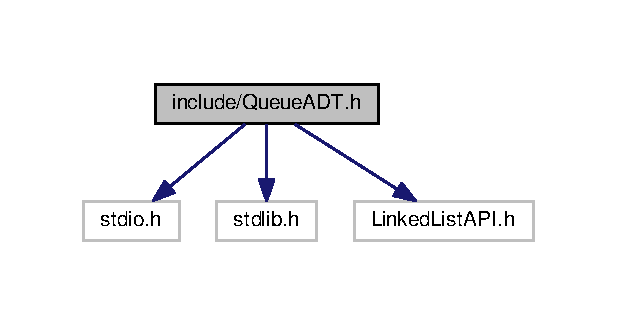
\includegraphics[width=296pt]{QueueADT_8h__incl}
\end{center}
\end{figure}
\subsection*{Classes}
\begin{DoxyCompactItemize}
\item 
struct \hyperlink{structqueue}{queue}
\end{DoxyCompactItemize}
\subsection*{Typedefs}
\begin{DoxyCompactItemize}
\item 
typedef struct \hyperlink{structqueue}{queue} \hyperlink{QueueADT_8h_a8560ae2ddf510ea6643f85a929bffa48}{Queue}
\end{DoxyCompactItemize}
\subsection*{Functions}
\begin{DoxyCompactItemize}
\item 
\hyperlink{QueueADT_8h_a8560ae2ddf510ea6643f85a929bffa48}{Queue} $\ast$ \hyperlink{QueueADT_8h_ad4f29ef77837d019f60ae26efb2ee7e2}{initialize\+Queue} (void($\ast$print\+Function)(void $\ast$to\+Be\+Printed), void($\ast$delete\+Function)(void $\ast$to\+Be\+Deleted), int($\ast$compare\+Function)(const void $\ast$first, const void $\ast$second))
\item 
void \hyperlink{QueueADT_8h_a8c22894fe355fc7eea3af009a8d41867}{delete\+Queue} (\hyperlink{QueueADT_8h_a8560ae2ddf510ea6643f85a929bffa48}{Queue} $\ast$\hyperlink{structqueue}{queue})
\item 
void \hyperlink{QueueADT_8h_af51b2730757b0b85ef389659909c64a6}{en\+Queue} (\hyperlink{QueueADT_8h_a8560ae2ddf510ea6643f85a929bffa48}{Queue} $\ast$\hyperlink{structqueue}{queue}, void $\ast$to\+Be\+Added)
\item 
void $\ast$ \hyperlink{QueueADT_8h_ab63d17936f81189aa01a9371c67d1745}{de\+Queue} (\hyperlink{QueueADT_8h_a8560ae2ddf510ea6643f85a929bffa48}{Queue} $\ast$\hyperlink{structqueue}{queue})
\item 
void $\ast$ \hyperlink{QueueADT_8h_ab3741001a45bf0fd0ceb260ce86527bd}{peek\+Queue} (\hyperlink{QueueADT_8h_a8560ae2ddf510ea6643f85a929bffa48}{Queue} $\ast$\hyperlink{structqueue}{queue})
\item 
void \hyperlink{QueueADT_8h_aa3e18bd8ba406c1ef7d07eb21f003091}{print\+Queue} (\hyperlink{QueueADT_8h_a8560ae2ddf510ea6643f85a929bffa48}{Queue} $\ast$\hyperlink{structqueue}{queue})
\end{DoxyCompactItemize}


\subsection{Detailed Description}
File containing the function definitions of a queue wrapping a doubly linked list. 

\begin{DoxyAuthor}{Author}
Ralph Arvin De Castro 
\end{DoxyAuthor}
\begin{DoxyDate}{Date}
June 2018 
\end{DoxyDate}


\subsection{Typedef Documentation}
\mbox{\Hypertarget{QueueADT_8h_a8560ae2ddf510ea6643f85a929bffa48}\label{QueueADT_8h_a8560ae2ddf510ea6643f85a929bffa48}} 
\index{Queue\+A\+D\+T.\+h@{Queue\+A\+D\+T.\+h}!Queue@{Queue}}
\index{Queue@{Queue}!Queue\+A\+D\+T.\+h@{Queue\+A\+D\+T.\+h}}
\subsubsection{\texorpdfstring{Queue}{Queue}}
{\footnotesize\ttfamily typedef struct \hyperlink{structqueue}{queue} \hyperlink{QueueADT_8h_a8560ae2ddf510ea6643f85a929bffa48}{Queue}}

Queue. It contains a list pointer, a node pointer that points to the front of the queue and length that determines number of elements. 

\subsection{Function Documentation}
\mbox{\Hypertarget{QueueADT_8h_a8c22894fe355fc7eea3af009a8d41867}\label{QueueADT_8h_a8c22894fe355fc7eea3af009a8d41867}} 
\index{Queue\+A\+D\+T.\+h@{Queue\+A\+D\+T.\+h}!delete\+Queue@{delete\+Queue}}
\index{delete\+Queue@{delete\+Queue}!Queue\+A\+D\+T.\+h@{Queue\+A\+D\+T.\+h}}
\subsubsection{\texorpdfstring{delete\+Queue()}{deleteQueue()}}
{\footnotesize\ttfamily void delete\+Queue (\begin{DoxyParamCaption}\item[{\hyperlink{QueueADT_8h_a8560ae2ddf510ea6643f85a929bffa48}{Queue} $\ast$}]{queue }\end{DoxyParamCaption})}

Deletes the queue from front, starting with the nodes, then list, then queue itself. \begin{DoxyPrecond}{Precondition}
\textquotesingle{}Queue\textquotesingle{} type must exist. 
\end{DoxyPrecond}
\begin{DoxyPostcond}{Postcondition}
Nodes,list and queue are deleted and freed. 
\end{DoxyPostcond}

\begin{DoxyParams}{Parameters}
{\em queue} & pointer to a queue \\
\hline
\end{DoxyParams}
\mbox{\Hypertarget{QueueADT_8h_ab63d17936f81189aa01a9371c67d1745}\label{QueueADT_8h_ab63d17936f81189aa01a9371c67d1745}} 
\index{Queue\+A\+D\+T.\+h@{Queue\+A\+D\+T.\+h}!de\+Queue@{de\+Queue}}
\index{de\+Queue@{de\+Queue}!Queue\+A\+D\+T.\+h@{Queue\+A\+D\+T.\+h}}
\subsubsection{\texorpdfstring{de\+Queue()}{deQueue()}}
{\footnotesize\ttfamily void$\ast$ de\+Queue (\begin{DoxyParamCaption}\item[{\hyperlink{QueueADT_8h_a8560ae2ddf510ea6643f85a929bffa48}{Queue} $\ast$}]{queue }\end{DoxyParamCaption})}

Removes a Node to the end of a queue \begin{DoxyReturn}{Returns}
void pointer that points to the deleted node 
\end{DoxyReturn}
\begin{DoxyPrecond}{Precondition}
\textquotesingle{}Queue\textquotesingle{} type must exist 
\end{DoxyPrecond}
\begin{DoxyPostcond}{Postcondition}
A node is removed and length decreases 
\end{DoxyPostcond}

\begin{DoxyParams}{Parameters}
{\em queue} & a pointer to a queue \\
\hline
\end{DoxyParams}
\mbox{\Hypertarget{QueueADT_8h_af51b2730757b0b85ef389659909c64a6}\label{QueueADT_8h_af51b2730757b0b85ef389659909c64a6}} 
\index{Queue\+A\+D\+T.\+h@{Queue\+A\+D\+T.\+h}!en\+Queue@{en\+Queue}}
\index{en\+Queue@{en\+Queue}!Queue\+A\+D\+T.\+h@{Queue\+A\+D\+T.\+h}}
\subsubsection{\texorpdfstring{en\+Queue()}{enQueue()}}
{\footnotesize\ttfamily void en\+Queue (\begin{DoxyParamCaption}\item[{\hyperlink{QueueADT_8h_a8560ae2ddf510ea6643f85a929bffa48}{Queue} $\ast$}]{queue,  }\item[{void $\ast$}]{to\+Be\+Added }\end{DoxyParamCaption})}

Inserts a Node to the end of a queue \begin{DoxyPrecond}{Precondition}
\textquotesingle{}Queue\textquotesingle{} type must exist and data to be added must exist 
\end{DoxyPrecond}
\begin{DoxyPostcond}{Postcondition}
A node is inserted and length increases 
\end{DoxyPostcond}

\begin{DoxyParams}{Parameters}
{\em queue} & a pointer to a queue \\
\hline
{\em to\+Be\+Added} & a pointer to data that is to be added to the linked list \\
\hline
\end{DoxyParams}
\mbox{\Hypertarget{QueueADT_8h_ad4f29ef77837d019f60ae26efb2ee7e2}\label{QueueADT_8h_ad4f29ef77837d019f60ae26efb2ee7e2}} 
\index{Queue\+A\+D\+T.\+h@{Queue\+A\+D\+T.\+h}!initialize\+Queue@{initialize\+Queue}}
\index{initialize\+Queue@{initialize\+Queue}!Queue\+A\+D\+T.\+h@{Queue\+A\+D\+T.\+h}}
\subsubsection{\texorpdfstring{initialize\+Queue()}{initializeQueue()}}
{\footnotesize\ttfamily \hyperlink{QueueADT_8h_a8560ae2ddf510ea6643f85a929bffa48}{Queue}$\ast$ initialize\+Queue (\begin{DoxyParamCaption}\item[{void($\ast$)(void $\ast$to\+Be\+Printed)}]{print\+Function,  }\item[{void($\ast$)(void $\ast$to\+Be\+Deleted)}]{delete\+Function,  }\item[{int($\ast$)(const void $\ast$first, const void $\ast$second)}]{compare\+Function }\end{DoxyParamCaption})}

Function to allocate memory to the struct, initialize list pointer, setting front to the the list of the head, initialize length to 0 \begin{DoxyReturn}{Returns}
pointer to the queue 
\end{DoxyReturn}

\begin{DoxyParams}{Parameters}
{\em print\+Function} & function pointer that prints a single node of the queue \\
\hline
{\em delete\+Function} & function pointer that deletes a single piece of data from the queue \\
\hline
{\em compare\+Function} & function pointer that compares two nodes of the list \\
\hline
\end{DoxyParams}
\mbox{\Hypertarget{QueueADT_8h_ab3741001a45bf0fd0ceb260ce86527bd}\label{QueueADT_8h_ab3741001a45bf0fd0ceb260ce86527bd}} 
\index{Queue\+A\+D\+T.\+h@{Queue\+A\+D\+T.\+h}!peek\+Queue@{peek\+Queue}}
\index{peek\+Queue@{peek\+Queue}!Queue\+A\+D\+T.\+h@{Queue\+A\+D\+T.\+h}}
\subsubsection{\texorpdfstring{peek\+Queue()}{peekQueue()}}
{\footnotesize\ttfamily void$\ast$ peek\+Queue (\begin{DoxyParamCaption}\item[{\hyperlink{QueueADT_8h_a8560ae2ddf510ea6643f85a929bffa48}{Queue} $\ast$}]{queue }\end{DoxyParamCaption})}

Looks at the data of the front of the queue \begin{DoxyReturn}{Returns}
void pointer that points to the data of the front node 
\end{DoxyReturn}
\begin{DoxyPrecond}{Precondition}
\textquotesingle{}Queue\textquotesingle{} type and front must exist 
\end{DoxyPrecond}

\begin{DoxyParams}{Parameters}
{\em queue} & a pointer to a queue \\
\hline
\end{DoxyParams}
\mbox{\Hypertarget{QueueADT_8h_aa3e18bd8ba406c1ef7d07eb21f003091}\label{QueueADT_8h_aa3e18bd8ba406c1ef7d07eb21f003091}} 
\index{Queue\+A\+D\+T.\+h@{Queue\+A\+D\+T.\+h}!print\+Queue@{print\+Queue}}
\index{print\+Queue@{print\+Queue}!Queue\+A\+D\+T.\+h@{Queue\+A\+D\+T.\+h}}
\subsubsection{\texorpdfstring{print\+Queue()}{printQueue()}}
{\footnotesize\ttfamily void print\+Queue (\begin{DoxyParamCaption}\item[{\hyperlink{QueueADT_8h_a8560ae2ddf510ea6643f85a929bffa48}{Queue} $\ast$}]{queue }\end{DoxyParamCaption})}

Prints the data of the nodes of queue from front to end \begin{DoxyPrecond}{Precondition}
\textquotesingle{}Queue\textquotesingle{} type and front must exist 
\end{DoxyPrecond}
\begin{DoxyPostcond}{Postcondition}
Data of nodes are printed accordingly 
\end{DoxyPostcond}

\begin{DoxyParams}{Parameters}
{\em queue} & a pointer to a queue \\
\hline
\end{DoxyParams}

%--- End generated contents ---

% Index
\backmatter
\newpage
\phantomsection
\clearemptydoublepage
\addcontentsline{toc}{chapter}{Index}
\printindex

\end{document}
